\chapter{Суда России и мира}
\label{ch:ships-chapter}

Данная глава посвящена судам, принадлежащих России и другим странам мира. Суда могут иметь различное назначение -- военное или гражданское. Гражданские суда используются во множестве задач: грузоперевозках, рыболовстве, туризме, разведке полезных ископаемых, спасательных работах, а также в спортивных, культурных и других целях. Для хранения такого большого объема информации о судах необходимо вести базы знаний. Одной из таких баз знания является Викиданные. Данная работа направлена на изучение хранимых в Викиданных объектов кораблей и оценке качества и полноты их описания.

\begin{marginfigure}[0.0cm]
    {
    \setlength{\fboxsep}{0pt}%
    \setlength{\fboxrule}{1pt}%
    \fcolorbox{gray}{gray}{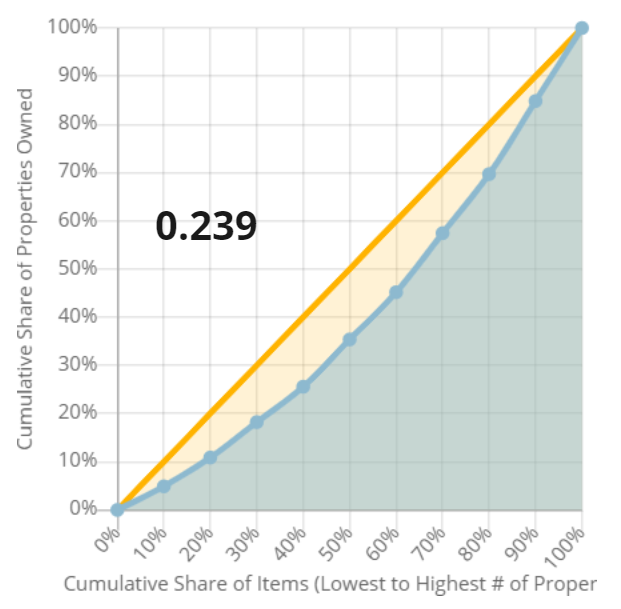
\includegraphics{../graphics/chapter/ship/Russian_ships_topic_imbalance.png}}
    }
      \caption{Низкая степень равномерности заполнения по числу свойств объекта Викиданных 
                    \href{https://www.wikidata.org/wiki/Q11446}{корабль (Q11446)}. 
                    Данные получены с помощью сервиса ProWD.id, 2020 год.
                    \emph{Коэффициент Джини равен 0.239.}}%
      \label{fig:prowd_ships-unbalanced}%
    \end{marginfigure}